\documentclass[11pt, a4paper]{article}

\usepackage{mlt-thesis-2015}

\usepackage[english]{babel}
\usepackage[hidelinks]{hyperref}
\usepackage{graphicx}
\usepackage{setspace}
\usepackage{comment}
\usepackage{caption}
\usepackage{listings}
\lstset{language=Pascal}

\usepackage[acronym]{glossaries}
\glsdisablehyper

\title{Visual question answering with type theory}
\subtitle{Using \gls{ttr} to model visual perception and language}
\author{Arild Matsson}
\date{}

\newacronym{hmm}{HMM}{Hidden Markov Model}
\newacronym{lstm}{LSTM}{Long Short-Term Memory}
\newacronym{cnn}{CNN}{convolutional neural network}
\newacronym{ttr}{TTR}{type theory with records}
\newacronym{nlg}{NLG}{natural language generation}
\newacronym{vqa}{VQA}{visual question answering}
\newacronym{yolo}{YOLO}{You only look once}
\newacronym{nlp}{NLP}{natural language processing}

\begin{document}

%% ============================================================================
%% Title page
%% ============================================================================
\begin{titlepage}

\maketitle

\vfill

\begingroup
\renewcommand*{\arraystretch}{1.2}
\begin{tabular}{l@{\hskip 20mm}l}
\hline
Master's Thesis: & 30 credits\\
Programme: & Master’s Programme in Language Technology\\
Level: & Advanced level \\
Semester and year: & Spring, 2018\\
Supervisors & Simon Dobnik and Staffan Larsson\\
Examiner & (name of the examiner)\\
Keywords & type theory, image recognition, object recognition, visual question answering
\end{tabular}
\endgroup

\thispagestyle{empty}
\end{titlepage}

%% ============================================================================
%% Abstract
%% ============================================================================
\newpage
\singlespacing
\section*{Abstract}

%\begin{abstract}
I'm connecting an off-the-shelf image recognition system to PyTTR, a Python implementation of TTR.
This enables representing concepts in the image as TTR types.
Then I'm implementing a \gls{vqa} task.
Questions are represented in TTR through really simple text parsing, and are answered using the representation of the image recognition results.
This shows that \gls{ttr} is helpful for representing visual perception, semantics and cognition.
\glsresetall
%\end{abstract}

\thispagestyle{empty}

%% ============================================================================
%% Preface
%% ============================================================================
\newpage
\section*{Preface}

Acknowledgements, etc.

\thispagestyle{empty}

%% ============================================================================
%% Contents
%% ============================================================================
\newpage

\begin{spacing}{0.0}
\tableofcontents
\end{spacing}

\thispagestyle{empty}

%% ============================================================================
%% Introduction
%% ============================================================================
\newpage
\setcounter{page}{1}

\section{Introduction}
\label{sec:intro}

(Just copied from the thesis proposal for now...)

This project will explore how \gls{ttr} can be used with an image recognition tasks such as question answering.
How can off-the-shelf image recognition software output be expressed in \gls{ttr}, and what can we do with it?

\begin{itemize}
\item Express image classification results in \gls{ttr}
\item Detect and recognize multiple objects in an image, as well as relationships between them
\begin{itemize}
\item Spatial, geometric relationships such as "above" and "to the left of"
\end{itemize}
\item Question anwering: parsing questions or statements into \gls{ttr} and judging their validity in relation to an image
\end{itemize}

\noindent
Development should focus on utilizing and possibly extending PyTTR, a Python implementation of \gls{ttr} \citep{pyttr}. Image recognition and natural language parsing/generation should use existing solutions as far as possible.

\section{Background}
\label{sec:background}

\cite{BlackburnComputationalsemantics2003}:
FOPC for the win. But "other approaches are both possible and interesting".

\subsection{Perceptual semantics}

\cite{LoganComputationalAnalysisApprehension1996}:
Basic–deictic(–intrinsic) relations.
Perceptual–conceptual representation.
"Computational theory of apprehension": spatial indexing -> reference frame -> ... Instead, we move into the conceptual level, both in perception and language, and evaluate validity from there.
(Drawbacks?)
They present "evidence" for their theory, does that evidence contradict the present approach?

\cite{RegierGroundingspatiallanguage2001a}:
AVS
Four models. AVS.
Many experiments.
Spatial term ratings influenced by: proximal \& center-of-mass orientations, grazing line, distance.

\cite{PustejovskyPerceptualsemanticsconstruction1990}?

\subsection{Type theory}

\subsubsection{Type theory, semantics and \gls{nlp}}

\glsreset{ttr}
\subsection{\Gls{ttr}}

\citep{CooperRecordsRecordTypes2005}:
TTR combines lambda calculus, phrase structure grammar, (DRT), (situation semantics) (what are the latter)?

\gls{ttr} is a formal framework for semantics \citep{CooperRecordsRecordTypes2005}.
It has been employed to model natural language in the context of dialogue, situated agents and spoken language.

\subsubsection{Applications of \gls{ttr}}

\cite{DobnikModellinglanguageaction2012} model a robot that would move around and use laser range scanner or similar to collect points in space, group them into objects and detect spatial relations between them.
\Gls{ttr} is used throughout the model, accounting for perception and cognition.

\subsubsection{PyTTR}

\subsection{Visual object recognition}

\begin{figure}[h]
\label{fig:dogbike_annotated}
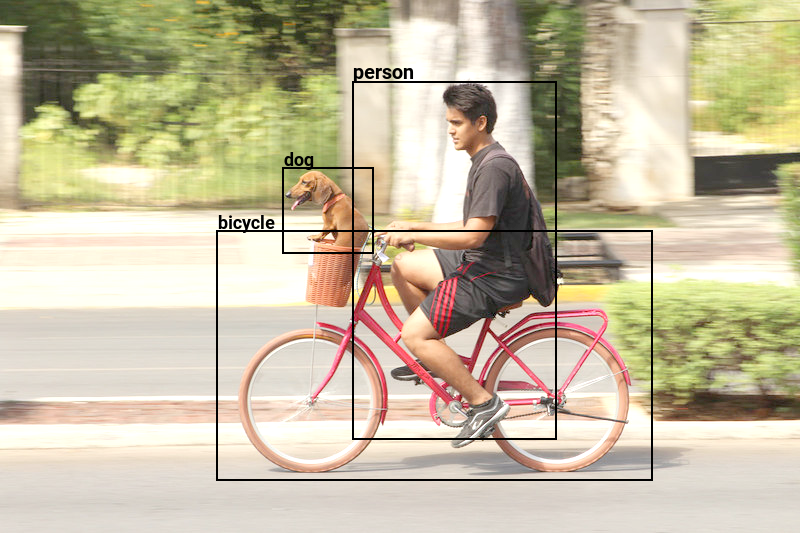
\includegraphics[width=\textwidth]{dogbike_annotated}
\centering
\caption{Visualization of labels and bounding boxes emitted by YOLO given an image depicting a cyclist with a dog.}
\end{figure}

\cite{Detectron2018}

\subsubsection{\Gls{vqa}}

\subsubsection{YOLO object recognition model}

You only look once (YOLO) \citep{RedmonYouOnlyLook2015} is a neural network model that simultaneously predicts bounding boxes around objects and classifies the contained objects.



\section{Method}
\label{sec:method}



\subsection{Theory development}

We looked at the suggestions put forward in LSPC and took it to the implementation stage.
Instead of pointspaces we used images.
To connect more with the linguistics of spatial semantics, we added simple parsing and validation of natural-language propositions/questions.

To collect the various parts as a united whole, we create an agent.



\subsubsection{Objects}

The three basic types $Int$ and $Image$ and $Ind$ are used to represent integers, 2D images and individual real-world objects, respectively.

A $Segment$ describes a rectangular bounding box as a record type:

\begin{equation}\label{eq:seg}
Segment = \left[\begin{array}{rcl}
\text{cy} &:& Int\\
\text{cx} &:& Int\\
\text{w} &:& Int\\
\text{h} &:& Int
\end{array}\right]\end{equation}

Functions of the type $Ppty$ can be applied to an individual and return a ptype depending on the individual, thus describing a property of it.

\begin{equation}\label{eq:ppty}
Ppty = (Ind \rightarrow Type)\end{equation}

An "object" is, at the perceptual level, modeled as a record of the type $Obj$, virtually a tuple of a position and a semantic property:

\begin{equation}\label{eq:obj}
Obj = \left[\begin{array}{rcl}
\text{seg} &:& Segment\\
\text{pfun} &:& Ppty \\
\end{array}\right]\end{equation}

For instance,

\begin{equation}\label{eq:objrec}
obj =
\left[\begin{array}{rcl}
\text{seg} &=& \left[\begin{array}{rcl}
\text{cx} &=& 138\\
\text{w} &=& 276\\
\text{cy} &=& 654\\
\text{h} &=& 809
\end{array}\right]\\
\text{pfun} &=& \lambda v:Ind\ .\ \text{person}(v)\\
\end{array}\right] : Obj\end{equation}

$Obj$ records are the result of performing \textit{object detection}.
This commitment is expressed in TTR as the function type $ObjDetector$:

\begin{equation}\label{eq:objdetector}
ObjDetector = ( Image \rightarrow [Obj] )
\end{equation}

At the conceptual level, an "object" is tied to a specific individual.
Because (reason?), we now use a record type, rather than a record, to model an object.
This is the \textit{basic relation} in \cite{LoganComputationalAnalysisApprehension1996}.

\begin{equation}\label{eq:indobj}
IndObj = \left[\begin{array}{rcl}
\text{x} &:& Ind \\
\text{loc} &:& Segment \\
\text{cp} &:& Type \\
\text{cl} &:& \text{location}(\text{x}, \text{loc}) \\
\end{array}\right]
\end{equation}

Had TTR allowed it, we could have been more specific by stating that the field $cp$ should be of a ptype dependent on the field $x$.

The step from the perceptual to the conceptual level is conducted by an \textit{individuation function}, a function of the type $IndFun$.

\begin{equation}\label{eq:indfun}
IndFun = ( Obj \rightarrow RecType )
\end{equation}

As a constraint that cannot be expressed in TTR, the record type resulting from applying an $IndFun$ function should be a subtype of $IndObj$.

So far, we have been following LSPC very closely.
But we also need $IndObj$ records (why, exactly?).
Thus, we let the record types created by the individuation function be \textit{fully specified}.



\subsubsection{Spatial relations}

Between any pair of individuals, a binary relation may take place.
Our concept of individuals is now a collection of fully specified $IndObj$ record types.
How do we detect and model a certain relation between such a pair?

Since we are interested in the spatial relation between a \textit{reference object} and a \textit{located object}, we will be constructing tuple-like records of the type $LocTup$:

\begin{equation}\label{eq:loctup}
LocTup = \left[\begin{array}{rcl}
    \text{lo} &:& IndObj \\
    \text{refo} &:& IndObj \\
    \end{array}\right]
\end{equation}

We model a classifier as a function from such a record to a new record type which should describe the relation:

\begin{equation}\label{eq:clf}
Clf = ( LocTup \rightarrow RecType )
\end{equation}

For instance, a classifier for "to the left of" might look like the following, where $\kappa_{left}$ is a non-TTR, boolean function algorithm with a boolean range.

\begin{equation}\label{eq:leftclfdef}
\lambda r : LocTup \ .\ 
\begin{cases}
\left[\begin{array}{rcl}
    \text{cr} &:& \text{left}(r.\text{lo}.\text{x}, r.\text{refo}.\text{x}) \\
\end{array}\right],
& \text{if } \kappa_{left}(r.\text{lo}.\text{loc}, r.\text{refo}.\text{loc}) \\
[], & \text{otherwise}
\end{cases}
\end{equation}



\subsubsection{Language}

A dog is to the left of a car
\begin{equation}\left[\begin{array}{rcl}
\text{x} &:& Ind\\
\text{y} &:& Ind\\
\text{c}_\text{dog} &:& \text{dog}(x)\\
\text{c}_\text{car} &:& \text{car}(y)\\
\text{c}_\text{left} &:& \text{left}(x, y)\\
\end{array}\right]\end{equation}


Essentially, we would like to check if the situation observed is a subtype of the situation described by the text/question, whether $Q \sqsupseteq A$. A new problem here is that field labels do not match, even if the field values (the types) match. We thus need to consider all (?) relabelings of $Q$:

A record type $T_1$ is a \textbf{relabel-subtype} of $T_2$, or $T_1 \sqsubseteq_{rlb} T_2$,  iff there is a relabeling of $T_1$, $T_{1_{rlb}}$ where $T_{1_{rlb}} \sqsubseteq T_2$.

(Or: iff $T_1$ is $\Sigma$-equivalent to a subtype of $T_2$?)

Could we forget field labels and just look at the two sets of field values? Not really, because we have dependent types, so $\text{dog}(x_1) ≠ \text{dog}(x_2)$. We need to carry out each candidate \textit{relabeling} and check subtypeness. In practice, and in this case, relabeling the basic-type ($Ind$) fields is enough, because those are the only ones whose labels appear in dependent fields. For each basic-field relabeling, we can then kind of forget labels and just find subtypeness of field values.

[Relabel-subtype pseudocode]



\subsubsection{Agent}

The perceptual-conceptual pieces described above are here combined.
We are building an agent who receives classified and located objects of an image, apprehends their basic status and spatial relations, and validates natural-language propositions.

\begin{equation}\label{eq:agent}
Agent = \left[\begin{array}{rcl}
    \text{objdetector} &:& ObjDetector \\
    \text{indfun} &:& IndFun \\
    \text{appr} &:& [(Rec \rightarrow RecType)] \\
    \text{state} &:& AgentState \\
    \end{array}\right]
\end{equation}

\begin{equation}\label{eq:state}
AgentState = \left[\begin{array}{rcl}
    \text{img} &:& Image \\
    \text{perc} &:& [Obj] \\
    \text{bel} &:& [RecType] \\
    \text{utt} &:& RecType \\
    \end{array}\right]
\end{equation}

The fields $objdetector$, $indfun$ and $appr$ of $Agent$ are to be statically defined for a specific agent.
While running, the agent will modify the $AgentState$ record in $state$.

\begin{enumerate}
\item Visual input in the form of an image is received and assigned to $state.img$.
\item $objdetector$ is invoked on $state.img$ and creates a collection of records that are assigned to $state.perc$.
\item $indfun$ is, in turn, invoked on each record in $state.perc$ and resulting record types are added to $state.bel$.
\item Now, the functions in $appr$ are applied to type-valid combinations of $state.bel$ records, and resulting record types are added to $state.bel$
	\begin{enumerate}
	\item Define "type-valid combinations"? How detailed?
	\end{enumerate}
\item Any language input is parsed and the resulting record type assigned to $state.utt$.
\item The record types in $state.bel$ are combined/concatenated. If the resulting record type is a relabel-subtype of $state.utt$, a positive answer is emitted; otherwise a negative answer is emitted.
\end{enumerate}



\subsection{Implementation}

Much of the theory developed above is straightforwardly implemented in PyTTR. 
Python is used mostly for binding the pieces together, but also some significant processes.



\subsubsection{Invoking YOLO}

YOLO is made with C but there is a Python wrapper.
When invoked from Python, the return value is a collection of dict objects with field for label, coordinates and a confidence score.
I made a Python function which takes this collection and translates it to a list of PyTTR $Obj$ records.

\begin{comment}
\begin{lstlisting}[language=Python]
from darkflow.net.build import TFNet
import numpy as np

tfnet = TFNet({"model": "yolo/yolo.cfg", "load": "yolo/yolo.weights",
    'config': 'yolo', "threshold": 0.2})

yolo_out = dict()
def yolo(img):
    """Invokes YOLO on a PIL image, caches and returns the result."""
    if str(img) not in yolo_out:
        yolo_out[str(img)] = tfnet.return_predict(np.array(img))
    return yolo_out[str(img)]

def yolo_coords(o):
    """Extract YOLO output coordinates as ((x0,y0), (x1,y1))."""
    return (o['topleft']['x'], o['topleft']['y']),
        (o['bottomright']['x'], o['bottomright']['y'])

def xy1xy2_to_cwh(x1, y1, x2, y2):
    '''Transform to center, width and height.'''
    return {'cx': int(x1/2 + x2/2), 'cy': int(y1/2 + y2/2),
        'w': x2 - x1, 'h': y2 - y1}

def yolo_detector(i):
    """Creates IndObj records for YOLO results."""
    return [Rec({
        'seg': Rec(xy1xy2_to_cwh(
            *yolo_coords(o)[0], *yolo_coords(o)[1])),
        'pfun': create_fun(o['label'].replace(' ', '_')),
    }) for o in yolo(i)] # @todo RBG/BGR?
ObjDetector.witness_cache.append(yolo_detector)
\end{lstlisting}
\end{comment}



\subsubsection{Spatial classifiers}

Spatial classifiers $\kappa$ are typed as $(Segment \rightarrow Segment \rightarrow bool)$.
I have implemented them as Python functions.
For the purpose of this thesis, no sophisticated spatial classification has been considered.
Instead, a naive comparison between centers of bounding boxes was implemented.
This was done for the four relations "left", "right", "above" and "below".



\subsubsection{Natural language parsing}

Parsing text to TTR has been addressed in \cite{CooperRecordsRecordTypes2005}, \cite{RobinCooperAustiniantruthattitudes2005}, \cite{CooperTypetheorysemantics2012}, \cite{CooperTypetheorylanguage2016}.
These accounts cover basic grammar, and are likely enough for the kind of utterances considered here.
It would have been interesting to see also those implemented here.
However, to save time I went for a simpler approach using NLTK's feature structure CFG.
With a custom Python function, the FOPC output is transformed to a TTR record type.



\subsubsection{Where PyTTR is not enough}

The individuation function, although expressible in TTR, is not possible to implement in PyTTR.
Therefore, it was implemented as a Python function named {\tt individualize}.
[Is the .create() usage also expressible in TTR?]

The \textit{relabel-subtype} relation, $\sqsubseteq_{rlb}$, was also implemented in Python.



\subsection{Evaluation}



\section{Results}
\label{sec:results}



\subsection{Limitations}

Disjunction ("or").



\section{Conclusions}
\label{sec:conclusions}



\subsection{Future work}

Basic->Deictic->Intrinsic relations  \cite{LoganComputationalAnalysisApprehension1996}

Spatial templates \& regions of acceptability. Compound relations (above right) finer (directly). Functional aspect.  \cite{LoganComputationalAnalysisApprehension1996} (also Dobnik etc)

4 question types.

Classification after Q.

Probabilistic TTR for "good fit" (is is more to the left or more above?).

Moar question types (tasks/programs/routines in L\&S).



\bibliography{imagettr}
\end{document}